% Three-page summary of the Part 1 report (E1 performance, E4 correctness).
% Build after analysis/part1_figures.py: latexmk -pdf summary.tex
\documentclass[10pt,a4paper]{article}
\usepackage[a4paper,margin=1.8cm,top=1.6cm,bottom=1.7cm]{geometry}
\usepackage[T1]{fontenc}
\usepackage[utf8]{inputenc}
\usepackage{charter}
\usepackage[scaled=0.9]{helvet}
\usepackage{amsmath,amssymb}
\usepackage{microtype}
\usepackage{graphicx}
\usepackage{booktabs,tabularx,array}
\usepackage{xcolor}
\usepackage{tikz}
\usetikzlibrary{arrows.meta,positioning}
\usepackage[most]{tcolorbox}
\usepackage{enumitem}
\usepackage{caption}
\usepackage{float}
\usepackage[hidelinks]{hyperref}

\DeclareUnicodeCharacter{00B5}{\ensuremath{\mu}}
\DeclareUnicodeCharacter{00D7}{\ensuremath{\times}}
\DeclareUnicodeCharacter{2192}{\ensuremath{\rightarrow}}

\definecolor{mfour}{HTML}{2A78D6}
\definecolor{refc}{HTML}{1BAF7A}
\definecolor{optc}{HTML}{6250D6}
\definecolor{fmlkem}{HTML}{1BAF7A}
\definecolor{fhqc}{HTML}{EDA100}
\definecolor{ffrodo}{HTML}{E87BA4}
\definecolor{fmce}{HTML}{008300}
\definecolor{ink2}{HTML}{52514E}
\definecolor{muted}{HTML}{898781}
\definecolor{gridc}{HTML}{E1E0D9}
\definecolor{wash}{HTML}{F4F3EF}
\definecolor{good}{HTML}{006300}

\setlist{itemsep=0.5pt,topsep=2pt,parsep=0pt,leftmargin=1.1em}
\captionsetup{font=small,labelfont=bf,labelsep=period,skip=2pt}
\setlength{\parindent}{0pt}
\setlength{\parskip}{3pt}
\renewcommand{\arraystretch}{1.08}
\pagestyle{empty}
\newcommand{\key}[1]{\textbf{#1}}
\newcommand{\head}[1]{\par\vspace{5pt}{\sffamily\bfseries\large #1}\par\vspace{1pt}}
\newtcolorbox{takeaway}{colback=wash,colframe=wash,boxrule=0pt,arc=2pt,left=6pt,right=6pt,top=3pt,bottom=3pt}
\newcommand{\tile}[3]{\begin{tcolorbox}[colback=wash,colframe=wash,arc=3pt,left=6pt,right=6pt,top=4pt,bottom=4pt]
{\fontsize{15}{17}\selectfont\bfseries\sffamily #1}\par{\footnotesize\bfseries\sffamily #2}\par{\scriptsize\sffamily\color{ink2}#3}\end{tcolorbox}}

\newcommand{\fxMecdh}{62.5\,µs}
\newcommand{\relMecdh}{1}
\newcommand{\fxMmlkemI}{17.6\,µs}
\newcommand{\relMmlkemI}{0.28}
\newcommand{\invMmlkemI}{3.6}
\newcommand{\fxMmlkemIII}{28\,µs}
\newcommand{\relMmlkemIII}{0.45}
\newcommand{\invMmlkemIII}{2.2}
\newcommand{\fxMmlkemV}{42.4\,µs}
\newcommand{\relMmlkemV}{0.68}
\newcommand{\invMmlkemV}{1.5}
\newcommand{\fxMhybrid}{100\,µs}
\newcommand{\relMhybrid}{1.6}
\newcommand{\fxMhqcI}{3.41\,ms}
\newcommand{\relMhqcI}{55}
\newcommand{\fxMfrodoI}{2.72\,ms}
\newcommand{\relMfrodoI}{43}
\newcommand{\fxMmceI}{52.6\,ms}
\newcommand{\relMmceI}{841}
\newcommand{\fxIecdh}{115\,µs}
\newcommand{\relIecdh}{1}
\newcommand{\fxImlkemI}{20.8\,µs}
\newcommand{\relImlkemI}{0.18}
\newcommand{\invImlkemI}{5.5}
\newcommand{\fxImlkemIII}{33.2\,µs}
\newcommand{\relImlkemIII}{0.29}
\newcommand{\invImlkemIII}{3.5}
\newcommand{\fxImlkemV}{46.4\,µs}
\newcommand{\relImlkemV}{0.4}
\newcommand{\invImlkemV}{2.5}
\newcommand{\fxIhybrid}{191\,µs}
\newcommand{\relIhybrid}{1.7}
\newcommand{\fxIhqcI}{7.35\,ms}
\newcommand{\relIhqcI}{64}
\newcommand{\fxIfrodoI}{2.23\,ms}
\newcommand{\relIfrodoI}{19}
\newcommand{\fxImceI}{38.7\,ms}
\newcommand{\relImceI}{337}
\newcommand{\eFourVectors}{1,332}
\newcommand{\eFourChecks}{69}


\tikzset{
  party/.style={draw=ink2,rounded corners=2pt,minimum width=1.9cm,minimum height=0.6cm,font=\sffamily\scriptsize\bfseries,fill=wash},
  op/.style={draw=ink2!70,rounded corners=2pt,font=\sffamily\scriptsize,fill=white,align=center,inner sep=2pt},
  msg/.style={-{Stealth[length=2mm]},thick,ink2},
  lbl/.style={font=\sffamily\scriptsize,ink2,align=center},
}

\begin{document}

% ------------------------------------------------------------------ page 1
{\sffamily\color{ink2}\small Cybersecurity Lab 1 · ELTE · Hamdan Al-Jabri · 11 October 2026}\par
{\sffamily\bfseries\LARGE Post-quantum KEMs: summary of Part 1}\par
{\sffamily\large\color{mfour} Performance (E1) and correctness (E4) on Apple M4 (ARM64) and Intel i7-1185G7 (x86-64)}\par
\vspace{4pt}

\begin{tcbraster}[raster columns=3,raster equal height,raster column skip=6pt,raster row skip=6pt]
\tile{\eFourChecks/\eFourChecks}{checks pass on both machines}{\eFourVectors{} vectors incl.\ NIST FIPS 203 (ACVP)}
\tile{\invMmlkemIII× / \invImlkemIII×}{ML-KEM-768 cheaper than X25519}{full key exchange, M4 / i7}
\tile{\relMhybrid× / \relIhybrid×}{hybrid X25519MLKEM768 vs X25519}{= its two parts added together}
\tile{\relMfrodoI–\relMmceI×}{conservative KEMs vs X25519}{HQC, FrodoKEM, McEliece, level 1 (M4)}
\tile{25–16,000×}{more bytes than X25519}{ML-KEM-768: 2,272\,B vs 64\,B}
\tile{up to 1,400×}{speed-up from AVX2 code}{McEliece decaps; NEON only for ML-KEM}
\end{tcbraster}

\head{1\quad Why these four KEMs}
One KEM from each corner of a $2\times2$ map, so that the comparison isolates both the \emph{family} (lattice vs.\ code) and the price of \emph{dropping algebraic structure}:

\begin{center}\small
\begin{tabularx}{\linewidth}{@{}l l l>{\raggedright\arraybackslash}X@{}}
\toprule
KEM & family / structure & status (Oct 2026) & role in the study\\
\midrule
\textcolor{fmlkem!80!black}{\textbf{ML-KEM}} & lattice, structured (Module-LWE) & NIST FIPS 203 (2024) & the standard; reference point\\
\textcolor{fhqc!80!black}{\textbf{HQC}} & code, structured (quasi-cyclic) & NIST selected (2025) & NIST's backup with different maths\\
\textcolor{ffrodo!80!black}{\textbf{FrodoKEM}} & lattice, unstructured (plain LWE) & ISO/IEC 18033-2 Amd 2 (2026), BSI & ML-KEM without structure\\
\textcolor{fmce}{\textbf{Classic McEliece}} & code, unstructured (Goppa) & ISO (2026), BSI & most conservative; huge keys\\
\bottomrule
\end{tabularx}
\end{center}
Each at NIST levels 1, 3 and 5 (12 KEMs), against classical \key{X25519} and the deployed hybrid \key{X25519MLKEM768}.

\head{2\quad KEMs, and how Diffie–Hellman becomes one}
\begin{minipage}[t]{0.5\linewidth}
\vspace{0pt}
A \key{KEM} is three algorithms: $\mathsf{KeyGen}()\to(pk,sk)$; $\mathsf{Encaps}(pk)\to(ct,K)$; $\mathsf{Decaps}(sk,ct)\to K$. Both sides end with the same 32-byte key $K$ after one message each way.

Post-quantum schemes have no efficient Diffie–Hellman, so TLS carries KEMs in its key shares. \key{Ephemeral X25519 already has the KEM shape}: the client's key pair is KeyGen, the server's key pair + DH is Encaps, and the client's DH is Decaps. We time it that way (\key{X25519-ECDH}, as in TLS 1.3) and also as \key{DHKEM} (RFC 9180), which adds HKDF and costs 10–14\% more.

The \key{hybrid} sends ML-KEM's key share followed by X25519's (1,216 / 1,120\,B) and concatenates both secrets (64\,B).
\end{minipage}\hfill
\begin{minipage}[t]{0.47\linewidth}
\vspace{2pt}
\centering
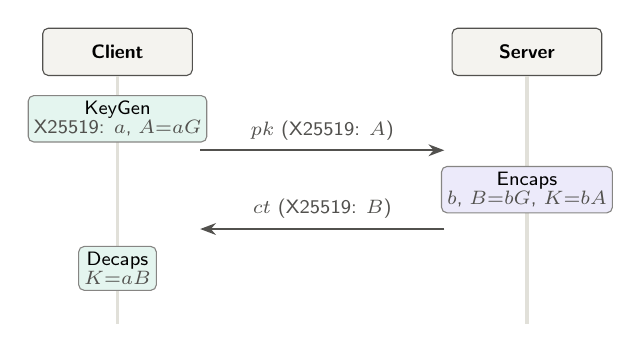
\begin{tikzpicture}
\node[party] (A) at (0,0) {Client};
\node[party] (B) at (5.2,0) {Server};
\draw[gridc,very thick] (A.south) -- ++(0,-3.15);
\draw[gridc,very thick] (B.south) -- ++(0,-3.15);
\node[op,fill=refc!12] at (0,-0.85) {KeyGen\\[-1pt]\textcolor{ink2}{X25519: $a$, $A{=}aG$}};
\draw[msg] (1.05,-1.25) -- node[above,lbl]{$pk$ (X25519: $A$)} (4.15,-1.25);
\node[op,fill=optc!12] at (5.2,-1.75) {Encaps\\[-1pt]\textcolor{ink2}{$b$, $B{=}bG$, $K{=}bA$}};
\draw[msg] (4.15,-2.25) -- node[above,lbl]{$ct$ (X25519: $B$)} (1.05,-2.25);
\node[op,fill=refc!12] at (0,-2.75) {Decaps\\[-1pt]\textcolor{ink2}{$K{=}aB$}};
\end{tikzpicture}
\captionof{figure}{KEM roles, with plain X25519 mapped onto them.}
\end{minipage}

\head{3\quad Setup and choices}
\begin{itemize}
\item \key{Same software on both machines}: Ubuntu 24.04, GCC 13.3, liboqs 0.16.0, OpenSSL 3.5.8; only the CPU differs (M4 in Docker Desktop, i7 in WSL2).
\item \key{Three builds}: liboqs \texttt{ref} (portable C), liboqs \texttt{opt} (AVX2/NEON), OpenSSL (X25519, ML-KEM, hybrid). Optimised code exists for ML-KEM on both CPUs, for FrodoKEM and McEliece only on x86, for HQC on neither.
\item \key{Timing}: every call timed with the CPU counter, 1,000 calls per operation (McEliece keygen 100), \key{median} and IQR; per-run calibration, 200\,ms warm-up, 30\,s cooldown (fanless Air), core clock estimated so results can also be given in cycles.
\end{itemize}

\newpage
% ------------------------------------------------------------------ page 2
\head{4\quad E4: correctness}
\begin{takeaway}
\key{All \eFourChecks{} checks pass on both machines} (\eFourVectors{} vectors and round trips each): liboqs known-answer tests for all 12 KEMs in both builds, NIST ACVP FIPS 203 vectors for ML-KEM (360/360), random round trips, ref$\leftrightarrow$opt cross-checks, and liboqs$\leftrightarrow$OpenSSL ML-KEM interoperability. The optimised code computes exactly what the portable code does, on ARM64 and x86-64, so E1 compares like with like.
\end{takeaway}

\head{5\quad E1: what one key exchange costs}
\begin{figure}[H]
\centering
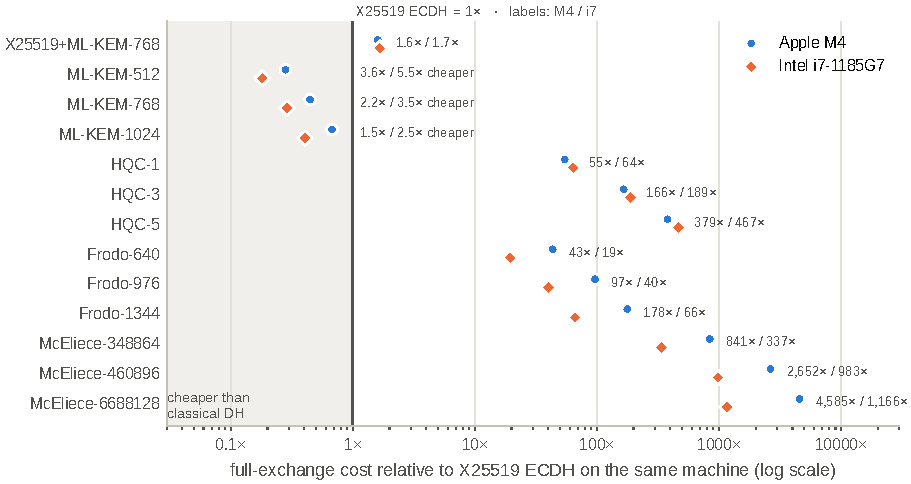
\includegraphics[width=0.93\linewidth]{fig/relative_to_x25519.pdf}
\caption{Compute for a full exchange (keygen + encaps + decaps, best build) relative to X25519 ECDH on the same machine.}
\end{figure}
\vspace{-4pt}
\begin{figure}[H]
\centering
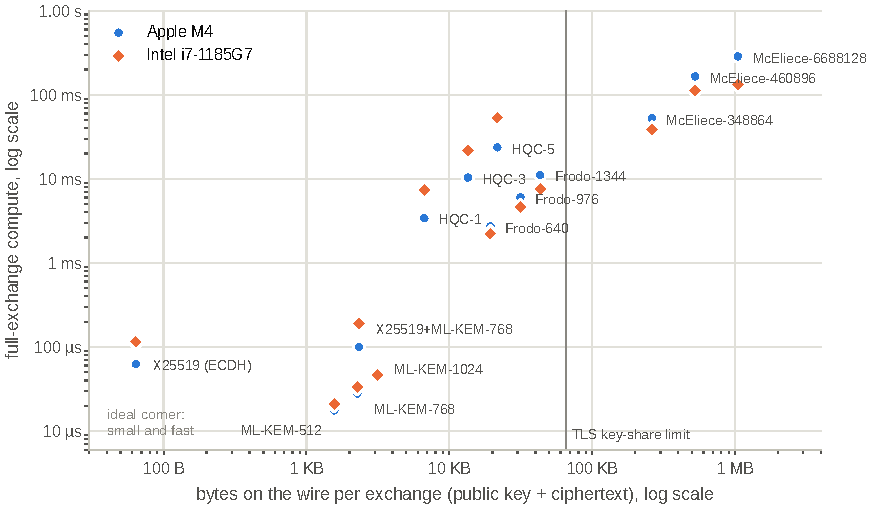
\includegraphics[width=0.93\linewidth]{fig/tradeoff.pdf}
\caption{Compute vs.\ bytes on the wire per exchange. Bottom-left is best; McEliece's public key exceeds the TLS limit.}
\end{figure}

\newpage
% ------------------------------------------------------------------ page 3
\begin{figure}[H]
\centering
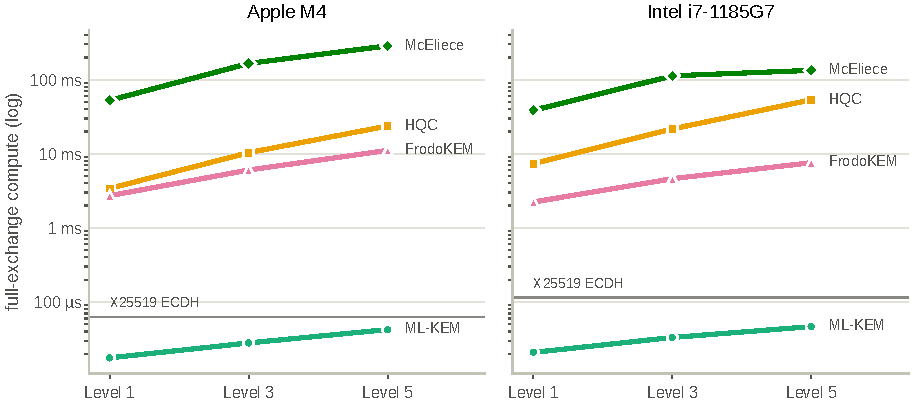
\includegraphics[width=0.74\linewidth]{fig/levels.pdf}
\caption{Full-exchange compute from NIST level 1 to 5 (log scale): ML-KEM stays below X25519 even at level 5.}
\end{figure}
\vspace{-6pt}
\begin{figure}[H]
\centering
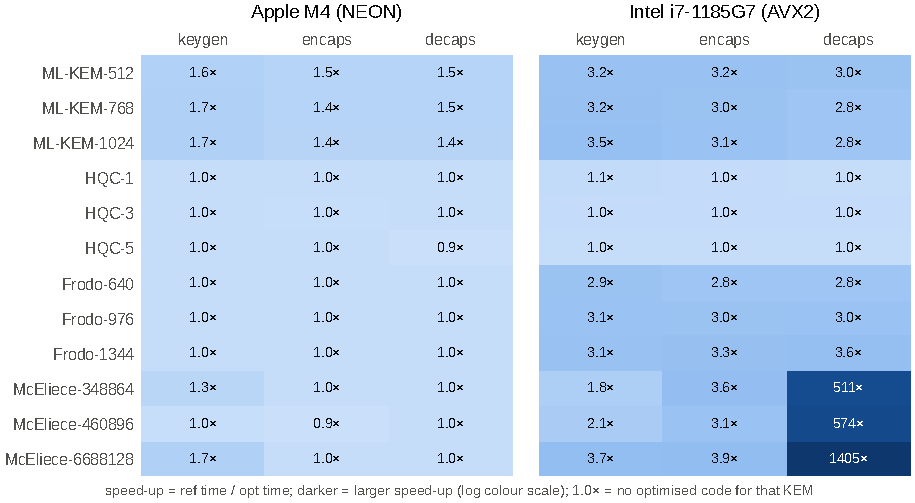
\includegraphics[width=0.8\linewidth]{fig/speedup.pdf}
\caption{Speed-up of optimised (AVX2 / NEON) over portable code; 1.0× = no optimised code for that KEM on that CPU.}
\end{figure}
\vspace{-4pt}
\head{6\quad Key findings}
\begin{enumerate}[leftmargin=1.4em]
\item \key{ML-KEM is cheaper than classical X25519} at every level: \invMmlkemIII× (M4) and \invImlkemIII× (i7) at level 3. It pays in bandwidth (25–49× more bytes), not CPU: small 12-bit arithmetic with the NTT vs.\ X25519's long chain of 255-bit multiplications.
\item \key{The hybrid costs \relMhybrid–\relIhybrid× X25519}, exactly X25519 plus ML-KEM: post-quantum TLS is cheap in compute.
\item \key{Conservative KEMs cost more in both dimensions}: at level 1 HQC \relMhqcI–\relIhqcI×, FrodoKEM \relIfrodoI–\relMfrodoI×, McEliece \relImceI–\relMmceI× the compute of X25519, with 4–14× ML-KEM's bytes (McEliece: 0.26–1\,MB public keys, too big for TLS).
\item \key{Implementation matters as much as the algorithm}: AVX2 speeds ML-KEM and FrodoKEM up $\sim$3× and McEliece decaps 510–1,400×; the M4 has NEON code only for ML-KEM (1.4–1.7×), so it beats the i7 by 2.2× on portable code but loses on FrodoKEM and McEliece. liboqs has no AVX2 HQC: the HQC team's own AVX2 code is 33–49× faster than what we measured.
\item \key{The i7 lowers its clock for AVX2 code} (3.9 $\to$ 3.2\,GHz); the fanless M4 stays at 4.0–4.44\,GHz with cooldowns. Results are also reported in core cycles for this reason.
\item \key{Validation}: HQC, McEliece encaps/decaps and the sizes match published figures; ML-KEM and FrodoKEM use fewer cycles than the 2021 spec code. Open: McEliece-348864 keygen is 2.6× the published cycle count.
\end{enumerate}

{\small\color{ink2}\textbf{Limitations:} Linux in a VM on both machines; one CPU per architecture; i7 time conversion varies 2.4\% between sessions (cycles unaffected). \textbf{Next (Part 2):} E2 TLS handshakes under delay and loss, E3 timing side channels. Full details and all tables: the 17-page Part 1 report. Code, data and figures: \texttt{github.com/hsh1994-ux/pq-kem-study}. Prepared with help from Claude (Anthropic); design and interpretation are the author's.\par}

\end{document}
